\section{Initial Maintenance and development guidelines}
\begin{itemize}
	\item First steps planning \\
		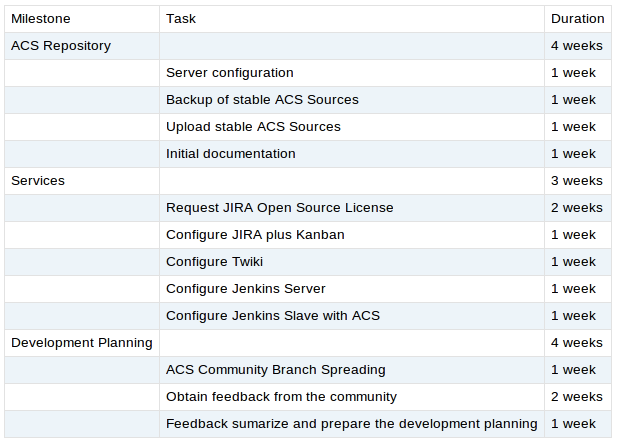
\includegraphics[width=0.65\textwidth]{img/planning.png}	
	\item Community Base Requirements
	\begin{itemize}
		\item Establish library dependencies: There is a problem in ACS to identify the dependencies for the modules/tools and external products. 
			Having this dependency tree will offer several benefits, for instance, it would facilitate the task of separating ACS into essential 
			parts, allowing to have a light version of ACS or putting it into RPM packages (or similar technologies) for easier distribution, etc. 
			It would also help in the learning curve of ACS by giving a way of navigating the different modules, knowing what are the list of 
			libraries involved in a program execution, which helps to isolate a problem to its root cause. Finally, having the list of 
			dependencies could be used to help the build process identify which sections require compilation and which can be skipped.
		\item Update external products and tools: Having the tools and external products updated could bring benefits for ACS. There are bug-fixes and 
			improvements, from which ACS can take advantage as well as support for newer platforms and build tools. Of course, along this benefits, 
			there are some costs that have to be considered, like upgrading patches created for older versions, building the newer versions, ensure 
			that new bugs that affect ACS aren't introduced, fixing API changes if they occur. To mitigate the situation where big changes occur when 
			updating the version of the products, a policy to periodically update them should be used, which should include documentation of the 
			benefits and problems that might be introduced, a set of tests if any bug is found in order to avoid regression problems. Updating all 
			the products simultaneously could be a big effort, and would be prominent to hide problems introduced between the tools. For this 
			reason, the update of the products should be done gradually or scheduled independently. In case that a new version of a tool 
			introduces unexpected new features/errors/deprecations/etc. the idea would be to patch the errors and find a workaround for unexpected 
			features/deprecations/etc. ACS maintenance for ALMA would be in charge of ESO, so the work in this branch would be independent of their
			development. The above doesn't mean that both projects could complement each other sharing features and bug-fixes.
		\item Plan to support more platforms: Having several supported platforms provides an easy way of distributing for several participants in the 
			community and increases the projects interested in using ACS by embracing their requirements. Having different supported platforms will 
			motivate the use of ACS by amateur projects, which enhances the use of a light version of ACS. Supporting more platforms doesn't come free, 
			however, as the time used in maintaining ACS increases. For this reason it is required to choose wisely how many and which platforms to 
			support. Additionally to maintenance there might be specific code required for some platforms which could produce code bloat.
		\begin{itemize}
			\item Windows
			\begin{itemize}
				\item Cygwin: There has been some work done to make ACS work with Cygwin under Windows. Currently ACS is built almost entirely and 
					behaves correctly on the core part of ACS, but some of the secondary features don't work as intended. This can be measured 
					considering the test results, which show us that around 70\% of the tests have a successful outcome.
				\item Native: There has been little work done to make ACS work natively on Windows using the Visual Studio compiler. All the External 
					Products and the Tools used by ACS were successfully built. Although ACS itself wasn't built and, for this reason, no tests 
					were made trying to run the system.
				\item Interested Projects: Windows is the operating system used by most people in the world. Therefore, providing support for this 
					system will automatically increase the opportunities to capture new projects to use ACS.
			\end{itemize}
			\item Mac: No work has been done to make ACS work under Mac, but we consider that this shouldn't be a hard task, since Mac is based on Unix 
				and provides most of the tools used by ACS.
			\begin{itemize}
				\item Interested Projects: There are several people interested in using Mac to develop with ACS and also there is a wide community 
					of amateur potential users that use Mac operating systems.
			\end{itemize}
			\item Several Linux Distributions: Currently Red Hat is the official operating system supported by ACS along with Scientific Linux which is 
				an alternative for this OS. Some work has been done to support ACS under different Linux platforms, which has led to working versions 
				of ACS under Fedora 14-16 and Ubuntu 8.04. As each operating system has its advantages and disadvantages, we shall offer alternatives 
				to the users. Considering the level of usage of the different versions of Linux by the community, we consider that the following 
				should be evaluated for support:
			\begin{itemize}
				\item Red Hat - Scientific Linux, Fedora, Ubuntu, Debian, Arch.
				\item Interested Projects: All the current projects that make use of ACS are currently using some variant of Linux, most probably Red 
					Hat or Scientific Linux. We can increase the interested projects by offering more alternatives to them.
			\end{itemize}
			\item Others (VxWorks, Solaris, HP-UX, etc.)
		\end{itemize}
		\item Plan to support more programming languages: Enhances the development of new services and tools for ACS by integrating more members of the 
			community and offering access to more libraries and integrated development environments such as .NET, Ruby on rails, etc. which offers help 
			for developing things like graphical user interfaces. On the other hand there is a lot of work to be done for implementing the infrastructure 
			for a new language to provide the services and the tools required for it.
		\item Specific GCC dependency: There is no specific dependency with GCC, although most of the code in the ACS Makefile is oriented for GCC.
		\item Compiling tools: It is possible to use different compilers either by using a compiler wrapper, or by modifying the 
			ACS Makefile. There have been some successful tests using Visual Studio compiler with the ACS Makefile for example.
		\item CUDA / OPENCL support: It should be possible to integrate ACS with parallel computing technologies.
	\end{itemize}
	\item Development
	\begin{itemize}
		\item DDS as Notification Channel: The idea is to use and extend the DDS wrapper library implemented by SPARTA project, to allow using different DDS 
			implementations, in spite of the missing standardization. SPARTA uses it for Real-Time Innovations (RTI) but keeps the option of switching it 
			in the future. ACS has extended it for OpenSplice, so far this library exists in C++ only. The task of this layer is not only to remove 
			dependencies on particular DDS implementations from the project code, but also to unify configuration of Quality of Services (QoS). 
		\item BACI Properties
		\begin{itemize}
			\item Java and Python full support
			\item Additional requirements: Depends on the feedback, could be new members, features, precision for BACI Properties, support additional 
				types, etc.
		\end{itemize}
		\item Code generator: Model Driven Architecture (MDA) software design approach is highly appraised when the project at hand has a big size. It aims
			at faster development, better communication across all levels of software, specifications and code re-usability. All these features help in
			decreasing the development time and the lines of code implemented, reducing human coding errors. 
		\item Simplify GUI creation process (Code Generation / Useful Widget Implementations / etc)
	\end{itemize}
\end{itemize}
